% ------------------------------------------------------------------------------
% TYPO3 CMS 6.2 LTS - What's New - Chapter "Risponsiv slike" (Serbian Version)
%
% @author	Sinisa Mitrovic <mitrovic.sinisaa@gmail.com>
% @license	Creative Commons BY-NC-SA 3.0
% @link		http://typo3.org/download/release-notes/whats-new/
% @language	Serbian
% ------------------------------------------------------------------------------
% Chapter: Risponsiv slike
% ------------------------------------------------------------------------------

\section{Risponsiv slike}
\begin{frame}[fragile]
	\frametitle{Risponsiv slike}

	\begin{center}\huge{Poglavlje 2:}\end{center}
	\begin{center}\huge{\color{typo3darkgrey}\textbf{Risponsiv slike}}\end{center}

\end{frame}

% ------------------------------------------------------------------------------
% Select Screen Size In Page Preview
% ------------------------------------------------------------------------------

\begin{frame}[fragile]
	\frametitle{Risponsiv slike}
	\framesubtitle{Izbor velicine ekrana u Page Preview}

	\begin{itemize}
		\item Urednici mogu odabrati razlicite velicine ekrana pomocu modula "View" da testiraju risponsiv sajtove
	\end{itemize}

	\begin{figure}
		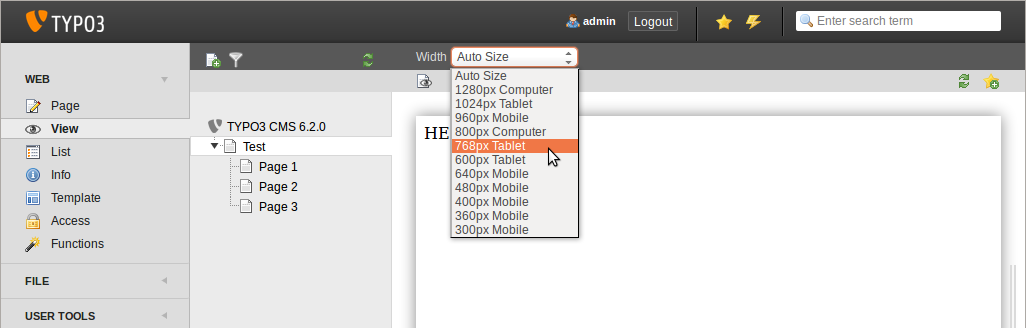
\includegraphics[width=0.95\linewidth]{Images/ResponsiveImages/ScreenSizeInPagePreview.png}
	\end{figure}

\end{frame}

% ------------------------------------------------------------------------------
% Customize Available Screen Sizes
% ------------------------------------------------------------------------------

\begin{frame}[fragile]
	\frametitle{Risponsiv slike}
	\framesubtitle{Prilagodjavanje posltojecih velicina ekrana}

	\begin{itemize}
		\item Velicine ekrana se mogu podesiti preko PageTSconfig:

		\lstset{
			basicstyle=\fontsize{7}{9}\selectfont\ttfamily
		}

		\begin{lstlisting}
			mod.web_view.previewFrameWidths {
			  1780.label = <any LLL or string>
			  1780.height = 145
			}
		\end{lstlisting}

		\item Sirina se odredjuje pomocu kljuca (ovde: 1780), visina je opciona
		\item Predefinisane velicine se mogu naci u fajlu:\newline
			\small\texttt{typo3/sysext/core/Configuration/DefaultConfiguration.php}\normalsize
		\item Naslovi se mogu definisati preko PageTSconfig:

		\begin{lstlisting}
			mod.web_view.previewFrameWidths {
			  1280.label = LLL:EXT:viewpage/Resources/Private/Language/locallang.xlf:computer
			  1024.label = LLL:EXT:viewpage/Resources/Private/Language/locallang.xlf:tablet
			}
		\end{lstlisting}

	\end{itemize}

\end{frame}

% ------------------------------------------------------------------------------
% Responsive Image Galleries
% ------------------------------------------------------------------------------

\begin{frame}[fragile]
	\frametitle{Risponsiv slike}
	\framesubtitle{Risponsiv galerije slika}

	\begin{itemize}
		\item Dodate su nove osobine za implementaciju risponsiv galerija slika
		\item "CSS styled content" je prosiren da bi se ovo postiglo
		\item Primer: HTML5 (zahteva \texttt{config.doctype = html5})\newline

			TYPO3 CMS < 6.2:

			\lstset{
				basicstyle=\fontsize{7}{9}\selectfont\ttfamily
			}

			\begin{lstlisting}
				<div class="csc-textpic-imagewrap">...</div>
			\end{lstlisting}

			TYPO3 CMS >= 6.2:

			\begin{lstlisting}
				<div class="csc-textpic-imagewrap"
				  data-csc-images="{register:imageCount}"
				  data-csc-cols="{field:imagecols}">...</div>
			\end{lstlisting}

	\end{itemize}

\end{frame}

% ------------------------------------------------------------------------------
% Responsive Image Rendering
% ------------------------------------------------------------------------------

\begin{frame}[fragile]
	\frametitle{Risponsiv slike}
	\framesubtitle{Renderanje risponsiv slika}

	\begin{itemize}
		\item cObject IMAGE rendera takozvani"sourceCollection" da bi podrzao razlicite dimenzije
		\item Renderanje risponsiv slika za cObject-e "text/image" i "image" zahteva dva podesavanja u Constant Editor:

			\texttt{styles.content.imgtext.responsive}\newline
			\texttt{styles.content.imgtext.layoutKey}

		\item Prihvatljive ("out of the box") opcije su:

			\begin{itemize}
				\item \texttt{default}:	\tabto{2cm} podrazumevani \texttt{<img>}-tag
				\item \texttt{srcset}:	\tabto{2cm} \texttt{<img>}-tag sa dodatnim izvorima kao srcset-atribut
				\item \texttt{picture}:	\tabto{2cm} \texttt{<picture>}-tag sa source-child-tagovima
				\item \texttt{data}:	\tabto{2cm} \texttt{<img>}-tag sa dodatnim izvorima kao data-atributi
			\end{itemize}

	\end{itemize}

\end{frame}

% ------------------------------------------------------------------------------
% Property: layoutKey
% ------------------------------------------------------------------------------

\begin{frame}[fragile]
	\frametitle{Risponsiv slike}
	\framesubtitle{Osobina: layoutKey}

	\begin{itemize}
		\item \texttt{layoutKey} definise renderanje layout-a\newline
			(ovo je HTML kod, koji se koristi za \texttt{<img>}-tag)
		\item Svaka opcija ima jedinstveno ponasanje za renderanje HTML-a
		\item Opcija \texttt{podrazumevana} rendera \texttt{<img>}-tag standardno\newline
			(ovo treba da se koristi ako sajt nije risponsiv)
		\item Implementiranje risponsiv layout-a zahteva razlicite dimenzije slika za razlicite rezolucije i velicine ekrana
		\item U zavisnosti od HTML framework-a, mogucnosti pretrazivaca i JavaScript biblioteka (za napredna poboljsanja):

			\begin{itemize}
				\item koristiti jedan od unapred definisanih layout-a
				\item definisati sopstveni layout
			\end{itemize}

	\end{itemize}

\end{frame}

% ------------------------------------------------------------------------------
% Property: layout
% ------------------------------------------------------------------------------

\begin{frame}[fragile]
	\frametitle{Risponsiv slike}
	\framesubtitle{Osobina: layout}

	\lstset{
		basicstyle=\tiny\ttfamily
	}

	\begin{lstlisting}
		layoutKey = {$styles.content.imgtext.layoutKey}
		layout {
		  default {
		    element = <img src="###SRC###" width="###WIDTH###" height="###HEIGHT###" ###PARAMS###
		      ###ALTPARAMS### ###BORDER######SELFCLOSINGTAGSLASH###>
		  }
		  srcset {
		    element = <img src="###SRC###" srcset="###SOURCECOLLECTION###" ###PARAMS###
		      ###ALTPARAMS### ###SELFCLOSINGTAGSLASH###>
		    source = |*|###SRC### ###SRCSETCANDIDATE###,|*|###SRC### ###SRCSETCANDIDATE###
		  }
		  picture {
		    element = <picture>###SOURCECOLLECTION###<img src="###SRC###" ###PARAMS###
		      ###ALTPARAMS######SELFCLOSINGTAGSLASH###></picture>
		    source = <source src="###SRC###" media="###MEDIAQUERY###"###SELFCLOSINGTAGSLASH###>
		  }
		  data {
		    element = <img src="###SRC###" ###SOURCECOLLECTION### ###PARAMS###
		      ###ALTPARAMS######SELFCLOSINGTAGSLASH###>
		    source = data-###DATAKEY###="###SRC###"
		  }
		}
	\end{lstlisting}

\end{frame}

% ------------------------------------------------------------------------------
% Property: layout.[layoutKey].element
% ------------------------------------------------------------------------------

\begin{frame}[fragile]
	\frametitle{Risponsiv slike}
	\framesubtitle{Osobina: layout.[layoutKey].element}

	\begin{itemize}
		\item \lstinline!###SRC###!\newline
			Atribut za URL: \texttt{src}

		\item \lstinline!###WIDTH###!\newline
			Atribut za sirinu slike (u pikselima): \texttt{width}

		\item \lstinline!###HEIGHT###!\newline
			Atribut za visinu slike (u pikselima): \texttt{height}

		\item \lstinline!###PARAMS###!\newline
			Dodatni parametri kao sto su definisani u cObject IMAGE

		\item \lstinline!###ALTPARAMS###!\newline
			Dodatni alternativni parametri kao sto su definisani u cObject IMAGE
	\end{itemize}

\end{frame}

% ------------------------------------------------------------------------------
% Property: layout.[layoutKey].element
% ------------------------------------------------------------------------------

\begin{frame}[fragile]
	\frametitle{Risponsiv slike}
	\framesubtitle{Osobina: layout.[layoutKey].element}

	\begin{itemize}
		\item \lstinline!###BORDER###!\newline
			Atribut za ivicu (u pikselima): \texttt{border}

		\item \lstinline!###SELFCLOSINGTAGSLASH###!\newline
			Zatvarajuci tag, na primer \texttt{<img ... />} nasuprot \texttt{<img ... >}\newline
			(zavisi od \texttt{config.xhtmlDoctype} ili \texttt{config.doctype})

		\item \lstinline!###SOURCECOLLECTION###!\newline
			Dodatni izvor slike, zavisi od koriscenja risponsiv dizajna.
			Tacne vrednosti su definisane u: \texttt{layout.[layoutKey].source}
	\end{itemize}

\end{frame}

% ------------------------------------------------------------------------------
% Property: sourceCollection.[dataKey]
% ------------------------------------------------------------------------------

\begin{frame}[fragile]
	\frametitle{Risponsiv slike}
	\framesubtitle{Osobina: sourceCollection.[dataKey]}

	\begin{itemize}
		\item Podrazumevan sourceCollection iz EXT:css\_styled\_content
		\item Pisanje sopstvenih sourceCollection-a je preporuceno

			\lstset{
				basicstyle=\tiny\ttfamily
			}

			\begin{lstlisting}
				sourceCollection {
				  small {
				    width = 200
				    srcsetCandidate = 600w
				    mediaQuery = (max-device-width: 600px)
				    dataKey = small
				  }
				  smallRetina {
				    if.directReturn = 1
				    width = 200
				    pixelDensity = 2
				    srcsetCandidate = 600w 2x
				    mediaQuery = (max-device-width: 600px) AND (min-resolution: 192dpi)
				    dataKey = smallRetina
				  }
				}
			\end{lstlisting}
	\end{itemize}

\end{frame}

% ------------------------------------------------------------------------------
% Further Resources (External Links)
% ------------------------------------------------------------------------------

\begin{frame}[fragile]
	\frametitle{Risponsiv slike}
	\framesubtitle{Dodatni resursi}

	\begin{itemize}
		\item Primeri koda:\newline
			\small\url{http://wiki.typo3.org/Responsive_Image_Rendering}\normalsize

		\item Artikl Sven Wolfermann-a na typo3.org:\newline
			\small\url{http://typo3.org/news/article/responsive-image-rendering-in-typo3-cms-62/}\normalsize

		\item W3C specification:\newline
			\small\url{http://www.w3.org/html/wg/drafts/srcset/w3c-srcset/}\newline
			\small\url{http://www.w3.org/TR/html-picture-element/}

		\item Working-Draft "Responsive Image Community Group":\newline
			\small\url{http://responsiveimages.org}\normalsize

	\end{itemize}

\end{frame}

% ------------------------------------------------------------------------------

